\chapter{Uppaal Modelling}
In the scope of this mini project we only choose to model some specific parts of the previously described steps.
Moreover, we do so in a slightly simplified manner.

The aspects we want to model are:
\begin{enumerate*}[label=\itshape\arabic*\upshape)]
    \item The process of joining the network;
    \item transmitting and receiving playback commands; and
    \item periodically synchronizing the slaves.
\end{enumerate*}
These roughly translates to~\ref{itm:connect},~\ref{itm:txrx}, and~\ref{itm:sync} from the aforementioned list of steps in the \textit{Introduction}.

\bigskip
To simplify the model and modelling process, we have some assumptions about the system, which does not reflect reality fully.
These are:
\begin{enumerate}[label=\itshape\arabic*\upshape)]
    \item All slaves will eventually try to connect to the master.
    \item The master cannot listen for incoming connection requests, while transmitting commands to devices already connected.
    \item Audio data, and the transmission or receiving of audio data, will not be considered in the model.
    \item The master transmits commands to the slaves sequentially, i.e.\ to one slave at a time.
    \item All slaves connected to the master will always receive transmitted commands.
    \item Synchronization of the slaves, is represented by a local boolean called \texttt{in\_sync}.
\end{enumerate}

Our system consists of two templates, one for the \textit{master} device and one for a \textit{slave}.
The system is instantiated with one master and five slaves.
In the following two sections we present the templates for the master and slave.

\section{Master Device}
The master device is the one which drives the system per say, and a system can only contain one master.

In~\ref{fig:master_model} the master model template can be seen.
The template consists of four color coded \enquote{zones}.
\begin{description}
    \item[\textcolor{orange}{The Orange Zone}] \hfill\\
        Represents the locations related to listening for slaves, which are trying to connect.
        The master will enter this zone when a slave request to join the network.
        The master will then either get a confirmation from the slave, or timeout and return to the \texttt{main\_idle} location.

    \item[\textcolor{blue}{The Blue Zone}] \hfill\\

\end{description}

\begin{figure}[ht]
    \centering
    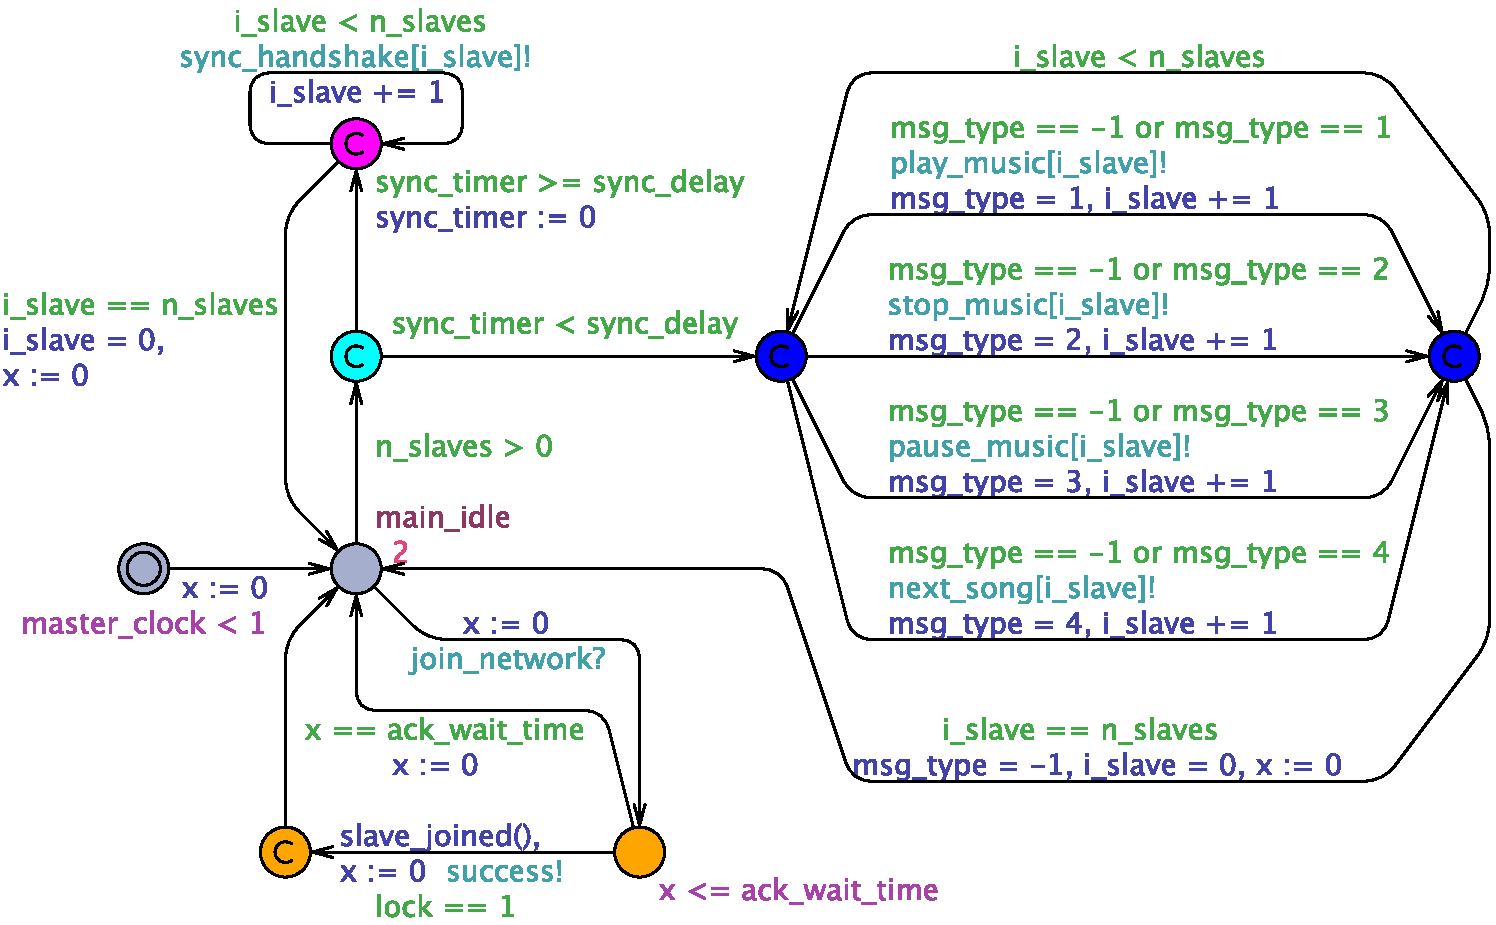
\includegraphics[width=1\textwidth]{master_model.pdf}
    \caption{Model of the \textit{master} device}\label{fig:master_model}
\end{figure}

\section{Slave Device}

\begin{figure}[ht]
    \centering
    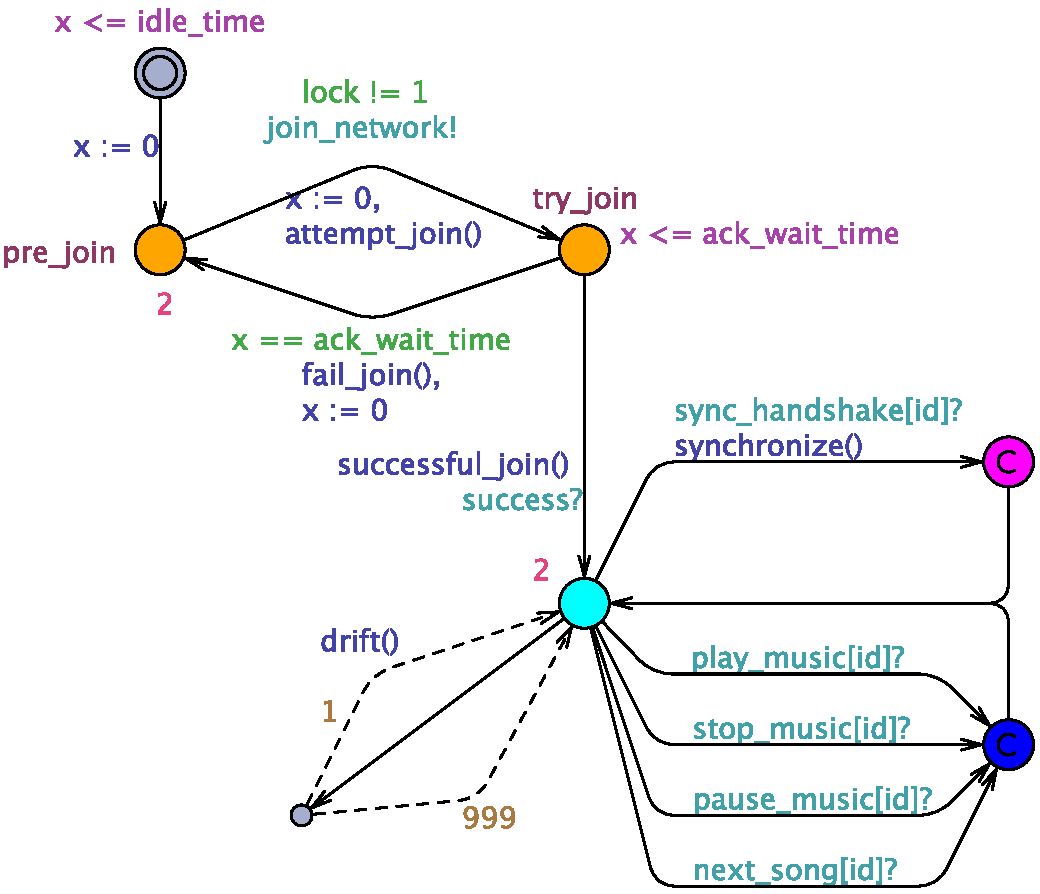
\includegraphics[width=0.75\textwidth]{slave_model.pdf}
    \caption{Model of a \textit{slave} device}
\end{figure}
This parts does something.

That part does something else.

Clocks and SMC!

